%%%%%%%%%%%%%%
% Fichero: AnteproyectoTFG
% Autor: Jesús Salido Tercero (http://www.uclm.es/profesorado/jsalido)
% Fecha (creación): Febrero 2014 
% Rev. : Febrero 2017
% Descripción: Plantilla para anteproyecto de TFG 
% (Escuela Sup. de Informática, UCLM). Creada para el curso 
% “LaTeX esencial para preparación de TFG, Tesis y otros documentos 
% académicos” (Esc. Sup. Informática-UCLM)
%
% Comentarios: Preparada para `pdflatex' y `biblatex' (con `biber'). 
% Documento editado con TeXstudio. 
% Para su compilación se aconseja utilizar como compilador 
% por defecto `latexmk.'
%%%%%%%%%%%%%%












\iffalse


% MEJORAS 

% MEJORAS REALIZADAS
[18:24, 6/12/2018] Jota A: no me gusta tu titulo
[18:24, 6/12/2018] Jota A: yo pondría lago como
[18:25, 6/12/2018] Jota A: Inteligencia artficial, sistemas expertos, sistemas basados en el conocimiento y minería de datos en el deporte de esgrima.
[18:25, 6/12/2018] Jota A: o
[18:25, 6/12/2018] Jota A: Aplicación de técnicas de inteligencia artficial, sistemas expertos, sistemas basados en el conocimiento y minería de datos en el deporte de esgrima.

[18:32, 6/12/2018] Jota A: página 4, en vez de hayo es halló
[18:37, 6/12/2018] Jota A: te falta la referencia de Scrum
[18:40, 6/12/2018] Jota A: falta referencia a drawio
[18:38, 6/12/2018] Jota A: falta referencia a trello
[18:38, 6/12/2018] Jota A: Sprint: periodo de tiempo entre una y cuatro semanas en las cual se divide un proyecto basado en Scrum


[18:39, 6/12/2018] Jota A: no entiendo porque hay varios sprints que tienen el mismo nombre
[18:39, 6/12/2018] Jota A: el sprint 0 no lo pongas, y si lo pones solo se usa para realizar la estimación de tiempo y tal
[18:40, 6/12/2018] Jota A: si en ese sprint hay trabajo real, entonces es sprint 1 no 0

[18:29, 6/12/2018] Jota A: revisa bien el capítulo de introducción
[18:29, 6/12/2018] Jota A: el punto 1 vaya
[18:29, 6/12/2018] Jota A: porque tienes fallos gramaticales, y creo que se puede redactar mucho mejor
[18:30, 6/12/2018] Jota A: por ej en vez de en marcha el plan trazando con anterioridad, pon: en marcha el plan trazado con anterioridad.




% MEJORAS PENDIENTES



[18:33, 6/12/2018] Jota A: un consejo que me dio Luis, es que no trates de mostrar mucho los puntos debiles del TFG, o sea, yo no pondría esto de Hay que tener en cuenta que al ser un prototipo tendrá un margen de error y no
será completo debido que trataremos las nociones básicas de la modalidad de espada. Una mejora en un futuro
que está fuera del alcance sería desarrollar esto mismo para las modalidades de forete y sable.
[18:33, 6/12/2018] Jota A: si quieres poner eso, ponlo en el apartado de trabajo futuro en la memoria final del TFG
[18:34, 6/12/2018] Jota A: aqui simplemente pon que se reducirá a lo de nociones básicas en espada y poco más
[18:34, 6/12/2018] Jota A: bueno, todo esto son consejos odviamente
[18:34, 6/12/2018] Jota A: haz lo que consideres más oportuno, o lo que de diga José Ángel


[18:41, 6/12/2018] Jota A: mete alguna referencia en el capítulo 1
[18:41, 6/12/2018] Jota A: y alguna más en el de metodología yo creo

[18:43, 6/12/2018] Jota A: y por cierto, en la memoria final del TFG pon alguna figura de gente compitiendo en esgrima, para situar al lector


\fi







% !TeX program = pdflatex

%%%%%%%%%%%%%%
% Preámbulo del documento
%%%%%%%%%%%%%%
\documentclass[11pt,a4paper,twoside,final]{article}
\usepackage[utf8]{inputenx} % Codificación de entrada
\usepackage[spanish,english]{babel} % Internacionalización
\usepackage{indentfirst} % Para asegurar sangrado en 1ª línea tras sección (necesario con varios idiomas)
\usepackage[top=2.5cm,bottom=2.5cm,inner=2cm,outer=2cm]{geometry}
\usepackage{float}
\raggedbottom

% Tipografía
\usepackage{libertine}
\usepackage[libertine]{newtxmath}


\usepackage{textcomp,marvosym,pifont} % Símbolos
\usepackage{cclicenses} % Para símbolos de licencias CC
\usepackage{amsmath,amsfonts,amssymb} % Caracteres matemáticos
\usepackage[T1]{fontenc} % Codificación de salida 
\usepackage{microtype} % Mejoras tipográficas para pdflatex

\usepackage{url} % Para escritura de URL
\urlstyle{sf}
\usepackage[bookmarks,hyperfootnotes=false,hidelinks]{hyperref}


% Definición de colores
% OJO: Este paquete debe cargarse antes de ctable. 
\usepackage[usenames,dvipsnames,svgnames,x11names,table]{xcolor}
\definecolor{sombra}{gray}{.70}


% Tablas y gráficos
\usepackage{ctable} % Inclusión de tablas. (ctable incluye): color,xkeyval,array,tabularx,booktabs,rotating
\usepackage{multirow}
\usepackage{graphicx}  % Inclusión de figuras
\graphicspath{{./figs/}} % Path de búsqueda de ficheros gráficos
\DeclareGraphicsExtensions{.pdf,.png,.jpg} % Precedencia de extensiones
\usepackage{rotating}  % Giro de cajas (texto, figuras, tablas) (No DVI)




% Ajustes de formato
\usepackage{paralist, multicol} % Mayor control de listas
\usepackage{titlesec} % Personalización completa de títulos de secciones
\usepackage{sectsty} % Personalización de títulos de sección con una interfaz más simple que la suministrada por titlesec
% Tipo de letra empleado en títulos de secciones (paquete sectsty)
\sectionfont{\sffamily\bfseries\MakeUppercase}
\subsectionfont{\sffamily\bfseries}
\subsubsectionfont{\sffamily\bfseries}
\usepackage[margin=10pt,font=small,labelfont=bf,format=hang]{caption} % Personalización de títulos de figuras y tablas



% !TeX TXS-program:bibliography = txs:///biber
% Bibliografía (Multilingüe en español e inglés, empleando el idioma de la fuente)
\usepackage[backend=biber,sortcites,autolang=other,language=auto]{biblatex}
% Línea añadida para eliminar el idioma de la fuente bibliográfica.
\AtEveryBibitem{\clearfield{note} \clearlist{language}}
\addbibresource{biblio.bib}
\usepackage[autostyle]{csquotes}







%====================================
%====================================

\begin{document}

%Selección de idioma principal del texto
\selectlanguage{spanish}




\begin{titlepage}
	\begin{center}
	
\includegraphics[width=3.5cm]{escudoInf}\\[1.5cm]
	 
	{\LARGE \textbf{UNIVERSIDAD DE CASTILLA-LA MANCHA \\[0.5em]
	ESCUELA SUPERIOR DE INFORMÁTICA}}\\[0.5cm]
	% EDITAR: Depto. del Director
	{\Large \textbf{Departamento de Tecnologías y Sistemas de Información}}\\[0.5cm]
	% EDITAR: Tecnología Específica Cursada
	{\large \textbf{Ciencias de la computación}}\\[1.5cm]
	{\LARGE \textbf{ANTEPROYECTO \\[0.5em]
	TRABAJO FIN DE GRADO}}\\[1cm]
	
	% EDITAR: Título de TFG	
	{\LARGE \textbf{Aplicación de técnicas de inteligencia artificial, sistemas expertos, sistemas basados en el conocimiento y minería de datos en el deporte de esgrima.}}\\[3cm]
	\end{center}
	
	% EDITAR: Nombre del autor y director(es)
	\begin{flushleft}
		{\Large Autor: Gregorio Baldomero Patiño Esteo} \\[1em]
		{\Large Director: Jose Angel Olivas Varela} \\[1em]
		% {\Large Director(a): Nombre y Apellidos} % Si no hay codirector comentar esta línea
	\end{flushleft}
	\vfill%
	
	% EDITAR: mes y año
	\begin{flushright}
		{\Large Noviembre, 2018}
	\end{flushright}
\end{titlepage}






%-> Índice General
\tableofcontents  % Índice general

\renewcommand{\tablename}{Tabla} % Se sustituye 'Cuadro' por 'Tabla'

\newpage

\section{Introducción}

En todo aspecto competitivo que te enfrente directamente a otra persona se tendrán que plantear diferentes estrategias para superar al rival. Estas estrategias se deciden a raíz del conocimiento sobre el deporte adquirido con el paso de los años y las experiencias vividas de cada persona. Además de esto hay otro componente principal a la hora de decantarse por una estrategia u otra, el adversario. Tomar estas decisiones no es nada fácil para una persona visto desde fuera, analizando todo lo que sucedió y pensando cuales serán los siguientes movimientos del rival. Una variable que aumenta la dificultad para esta toma de decisiones es tener que llevar a cabo estos pensamientos mientras intentas llevarlos a cabo. Esto pasa en los deportes individuales, has de pensar que hacer mientras pones en marcha el plan trazado con anterioridad.

\smallskip
Para ayudar en estas situaciones se inventó una figura de entrenador, la cuál ayudará a elegir una estrategia u otra en función de lo que se ve desde fuera, sin tener que preocuparse en llevar a cabo la anterior. De este modo al separar trabajos, mente y cuerpo, se podrá focalizar en cada uno de ellos y tener mayores probabilidades de obtener el éxito. Este caso sería el ideal pero a niveles bajos no se dispone de esta figura, por lo que resulta difícil sacar todo el potencial en competición.

\bigskip
El objetivo de este Trabajo de Fin de Grado (TFG a partir de ahora) consiste en desarrollar un entrenador virtual que sirva como apoyo en tiempo real para la toma de decisiones sobre estrategias en las competiciones de esgrima. También servirá para aquellas personas que quieran ampliar su conocimiento y saber que posibilidades hay ante diferentes situaciones en combate.

\bigskip
La elección del tema sobre el que versa este TFG surge a raíz de un problema visualizado durante las competiciones que no eran de alto nivel de esgrima. Solamente los tiradores de mas alto nivel tenían un entrenador personal que les pudiera ayudar, de este modo ellos solo se tenían que preocupar de llevar a cabo lo que les decían. Sin embargo el resto de tiradores tenían que pensar en que hacer a la vez que se tenían que defender del rival. De este modo en el momento que puedan consultar su teléfono móvil u ordenador portátil podrán hacer una consulta la cual les ayudará a tomar una decisión basándose en parámetros apreciables por el tirador, argumentando las razones y dando varias alternativas.

\newpage

\section{Tecnología específica cursada}
En el presente apartado se muestran dos tablas (Tabla 1 y Tabla 2) que indican respectivamente:
\begin{itemize}
    \item Tabla 1: La tecnología especifica / intensificación / itinerario cursado por el autor en su estancia en la ESI como alumno del Grado en Ingeniería en Informática.
    \item Tabla 2: Dentro de cada intensificación existen una serie de competencias para las cuales el alumno está capacitado, se muestran y explican cuáles de dichas competencias van a ser aplicadas durante el desarrollo de este TFG.
\end{itemize}

% Tratamiento de la tabla como un float
%\begin{table}[htb]
   %\centering
   %\caption{Tecnología Espécifica cursada por el alumno}
	 %\label{tab:tecno}
   %\rowcolors{1}{white}{sombra}
   %\begin{tabular}{cl}
		%\hline
          %& Tecnologías de la Información \\
          %& Computación   \\
          %& Ingeniería del Software \\
		%\ding{52}		& Ingeniería de Computadores \\
		%\hline
   %\end{tabular}
%\end{table}

% OJO: A petición de algunos alumnos he añadido un método poco ortodoxo para la creación de las tablas sin hacer uso de un entorno table. De este modo la tabla se incluye justo en el punto de su inclusión. El título y la numeración de la misma se incluye de modo "manual". En realidad este hack solo es preciso si la estructura final del documento es excepcionalmente rara con alguna sección en la que haya muy poco texto frente al tamaño de los elementos floats.

\begin{center}
   \textbf{Tabla 1}: Tecnología específica cursada por el alumno\\[1em]
   \rowcolors{1}{white}{sombra}
   \begin{tabular}{cl}
		\hline
          & Tecnologías de la Información \\
        \ding{52}  & Computación   \\
          & Ingeniería del Software \\
		  & Ingeniería de Computadores \\
		\hline
   \end{tabular}
\end{center}

\begin{center}
   \textbf{Tabla 2}: Justificación de las competencias específicas abordadas en el TFG\\[1em]
   \rowcolors{1}{white}{sombra}
   \begin{tabular}{p{.45\textwidth} p{.45\textwidth}}
		\textbf{Competencias} & \textbf{Justificación} \\
		\hline
			Capacidad para conocer y desarrollar técnicas de aprendizaje computacional y diseñar e implementar aplicaciones y sistemas que las utilicen, incluyendo las dedicadas a extracción automática de información y conocimiento a partir de grandes volúmenes de datos. & Durante el desarrollo de este TFG se ha generado una base de datos de la cual se ha extraído un modelo de aprendizaje automático con el que poder reforzar el entrenador.\\
			
            Capacidad para desarrollar y evaluar sistemas interactivos y de presentación de información compleja y su aplicación a la resolución de problemas de diseño de interacción persona computadora. & Se ha generado un aplicación mediante la cual un usuario puede interaccionar con ella para obtener respuestas a sus preguntas.\\
            
            Capacidad para adquirir, obtener, formalizar y representar el conocimiento humano en una forma computable para la resolución de problemas mediante un sistema informático en cualquier ámbito de aplicación, particularmente los relacionados con aspectos de computación, percepción y actuación en ambientes entornos inteligentes. &  Se ha formalizado conocimiento técnico y experiencia de un experto en la materia de esgrima y se ha plasmado en un programa como consecuente hemos obtenido un conjunto de reglas de las cuales mediante unas entradas se puede obtener una salida.  \\
            
			Capacidad para evaluar la complejidad computacional de un problema, conocer estrategias algorítmicas que puedan conducir a su resolución y recomendar, desarrollar e implementar aquella que garantice el mejor rendimiento de acuerdo con los requisitos establecidos. & Se han estudiado las complejidades de los algoritmos utilizados de modo que se halló la solución mas óptima para cada caso. \\
			
		\hline
   \end{tabular}
\end{center}


% Resto de competencias sin asignar.

%Capacidad para tener un conocimiento profundo de los principios fundamentales y modelos de la computación y saberlos aplicar para interpretar, seleccionar, valorar, modelar, y crear nuevos conceptos, teorías, usos y desarrollos tecnológicos relacionados con la informática.
%Capacidad para conocer los fundamentos, paradigmas y técnicas propias de los sistemas inteligentes y analizar, diseñar y construir sistemas, servicios y aplicaciones informáticas que utilicen dichas técnicas en cualquier ámbito de aplicación.


\newpage

\section{Objetivos}
%De acuerdo a la Introducción, el alumno deberá especificar cuál o cuáles son las hipótesis de trabajo de las que se parten, qué se pretende resolver, y en base a eso formular el objetivo principal delTFG.


%El objetivo principal deberá desglosarse en sub-objetivos parciales. Los sub-ojetivos deberán describirse de forma breve y concisa.

%Como preámbulo a la formulación del objetivo parcial, el alumno deberá discutir sobre las limitaciones y condicionantes a tener en cuenta en el desarrollo del TFG (lenguaje de desarrollo, equipos, madurez de la tecnología, etc.).

%Del mismo modo, será recomendable incluir una lista preliminar de requisitos del sistema a construir.

De acuerdo con la introducción dada al comienzo de este documento, el objetivo final de este TFG es desarrollar un prototipo de aplicación que sea capaz de dar una respuesta a ciertas situaciones planteadas durante un asalto de esgrima. Hay que tener en cuenta que al ser un prototipo tendrá un margen de error y no será completo debido que trataremos las nociones básicas de la modalidad de espada. Una mejora en un futuro que está fuera del alcance sería desarrollar esto mismo para las modalidades de florete y sable. Para ello se propone desarrollarlo en los siguientes sub-objetivos:

\begin{itemize}
    \item Desarrollar sistema experto. Para esta parte será necesario desarrollar las siguientes partes:
    \begin{itemize}
        \item Estudio de viabilidad. Este estudio será llevado a cabo mediante el test de Slagel.
        \item Adquisición de conocimiento. Se obtendrá conocimiento sobre el tema a tratar basandonose sobre todo en entrevistas a expertos de la materia.
        \item Conceptualización. Se plasmará de una forma entendible todo el conocimiento adquirido.
        \item Representación del conocimiento. Esta representación se mostrara en forma de reglas.
        \item Evaluación. Conclusiones del sistema experto.
    \end{itemize}
    \item Desarrollar modelo de aprendizaje para competiciones con base de datos.
    \begin{itemize}
        \item Adquisición datos.
        \item Tratamiento datos.
        \item Procesamiento datos.
        \item Obtener conocimiento.
    \end{itemize}
    \item Desarrollar aplicación juntando ambas partes anteriores.
    \begin{itemize}
        \item Alimentar sistema experto. Esto se hará con el conocimiento obtenido de los datos.
        \item Levantar servidor web. Para darle accesibilidad al programa desde cualquier sitio.
        \item Desarrollar página web. Para darle interfaz al programa.
        \item Conectar con sistema experto. Para que se pueda visualizar desde cualquier sitio con conexión a internet.
    \end{itemize}
\end{itemize}

El alcance de este proyecto está basado en el tiempo disponible para realizarlo. Varios autores han escrito libros para plasmar su conocimiento sobre este deporte, ya sea como plantear la gestión de un club, como preparar a los tiradores para competiciones, como iniciarlos, etc. Este último caso es el de Elain Cheris hablando sobre los fundamentos básicos de la esgrima en las modalidades de florete y espada ya que ambas comparten las bases. Este libro \textit{Manual de esgrima} \cite{manualdeesgrima} consta de 160 páginas en el que se habla sobre el primer año de aprendizaje de una persona que se inicia en el deporte. Para adquirir este conocimiento se requiere de muchas horas de trabajo y entrevistas con profesionales por lo que automáticamente descartamos la modalidad de sable, ya que hay poco conocimiento reutilizable.

\bigskip
Debido a los motivos expuestos anteriormente la modalidad de sable se dejará para un futuro lejano a modo de ampliación. Respecto a la modalidad de florete es cierto que comparten las bases pero las técnicas específicas y el conocimiento es totalmente distinto, por lo que se podrían utilizar partes del desarrollo pero toda la adquisición de conocimiento, desarrollo del sistema experto habría que realizarlo partiendo de cero. Para ambas modalidades hay que sumar que conseguir expertos resulta de gran dificultad actualmente, cosa que en un futuro lejano, tres años, espero solventar. Todo esto ha llevado a los objetivos expuestos anteriormente.


\newpage

\section{Métodos y fases de trabajo}

Durante mucho tiempo se ha seguido una metodología que dificultaba la adaptabilidad de un proyecto a futuros cambios. Se definía el proyecto al principio, capturando todos los requisitos necesarios, se planificaban y hasta que no se acabaran no podían incluirse nuevos y esto era haciendo de nuevo todo el ciclo. Esta metodología se llama en cascada y tiene el siguiente esquema:

\begin{figure}[H]
  \centering
   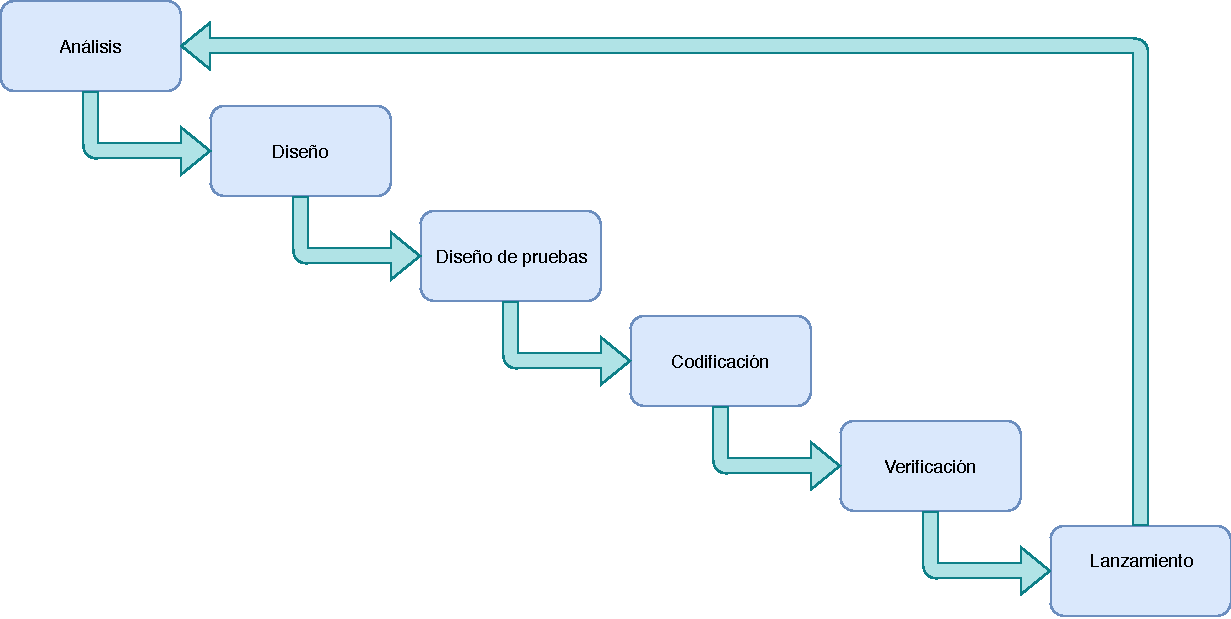
\includegraphics[width=0.7\textwidth]{Cascada.pdf}
   \caption{Ciclo cascada}
  \label{Ciclo cascada}
\end{figure}

Esta metodología es idónea para aquellos proyectos que se quieren dar fechas de entrega con mucha precisión, aquellos en los que se tiene claro desde el inicio que, como y cuando se va a hacer. La naturaleza de este TFG no permite que que se trabaje de esta manera debido a que es posible que se encuentren problemas durante el desarrollo del mismo y haya que buscar otras alternativas durante el mismo además de tener que repetir alguna de las fases con relativa frecuencia sin haber llegado a alguna de las siguientes. Como alternativa a este tipo de metodologías se diseño las metodologías ágiles, entre ellas SCRUM \cite{scrum} que será la elegida para este TFG.

SCRUM se basa en que se pueden hacer cambios en la planificación en cualquier momento. Se planifica la tarea para cada sprint \footnote{Sprint: periodo de tiempo entre una y cuatro semanas en las cual se divide un proyecto basado en Scrum} de tal modo que en función de la duración de este los cambios se podrán ir adaptando en función de la necesidad del proyecto en ese momento. Además, dado que es una metodología ágil, favorece los cambios de última hora, esto quiere decir que permite añadir, quitar o modificar el trabajo planificado para ese periodo de tiempo. Para ello se tiene una cola de tareas, ordenadas por prioridad las cuales se van metiendo en el sprint por orden. Debido a esto encaja perfectamente con las características del proyecto y será la metodología escogida para llevar a cabo el mismo. Al ser una metodología pensada para grupos de personas y este proyecto será llevado a cabo por una única persona se harán modificaciones sobre este mismo para adaptarlo.

Para hacernos una idea de cual es el ciclo de vida en un proyecto de scrum podemos observar la siguiente figura:

\begin{figure}[H]
  \centering
   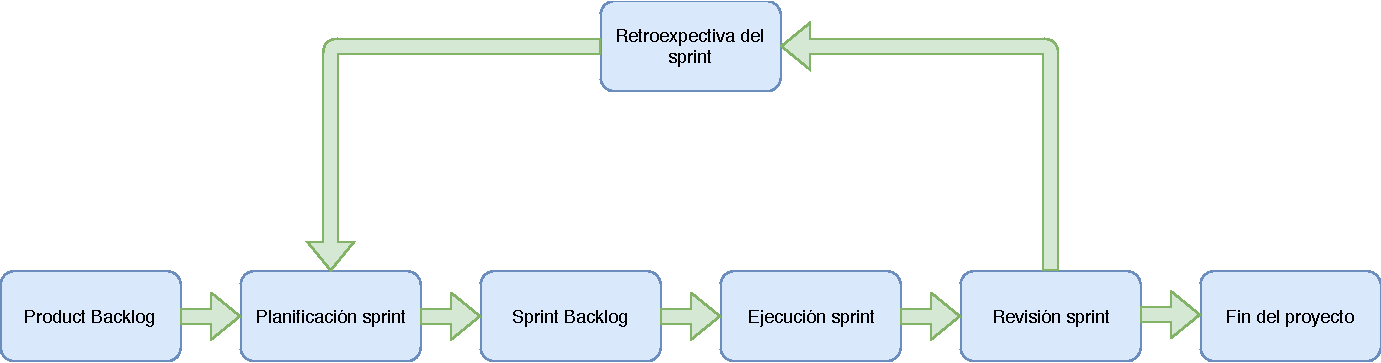
\includegraphics[width=0.7\textwidth]{Scrum.pdf}
  \caption{Ciclo SCRUM}
  \label{Ciclo SCRUM}
\end{figure}

Se eliminaron las reuniones diarias puesto que no tienen sentido en equipos de una persona, ya que no habrá bloqueos entre personas con sus tareas.

\bigskip

Para el product backlog se usará trello \cite{trello} ya que nos permite crear tablones con notas y estas notas serán las tareas a realizar, ordenadas de arriba a abajo según su prioridad. Además se usará esta plataforma para saber el avance de cada tarea. Cada tarea tendrá una checklist compuesta por tres elementos. Estos elementos servirán para indicar el estado de la tarea. Dichos elementos serán \textit{tarea de sprint}, \textit{en desarrollo} y \textit{terminada}. En la \textbf{tabla 3} se puede ver una estimación inicial de sprints teniendo estos una duración de tres semanas.


\begin{center}
   \textbf{Tabla 3}: Planificación estimada del proyecto\\[1em]
   \rowcolors{1}{white}{sombra}
   \begin{tabular}{p{.30\textwidth} p{.20\textwidth} p{.30\textwidth}}
        \hline
		\textbf{Línea temporal} & \textbf{Duración}  & \text{Temática}\\
		\hline
		    \textbf{14/01/2019 - 01/02/2019} & Sprint 1 & Desarrollo sistema experto\\
		    \textbf{04/02/2019 - 22/02/2019} & Sprint 2 & Desarrollo sistema experto \\
		    \textbf{25/02/2019 - 15/03/2019} & Sprint 3 & Desarrollo sistema experto y desarrollo modelo aprendizaje\\
		    \textbf{18/03/2019 - 05/04/2019} & Sprint 4 & Desarrollo modelo aprendizaje\\
		    \textbf{05/04/2019 - 26/04/2019} & Sprint 5 & Desarrollo modelo aprendizaje\\
		    \textbf{29/04/2019 - 17/05/2019} & Sprint 6 & Desarrollo modelo aprendizaje y Desarrollo aplicación web\\
		    \textbf{20/05/2019 - 07/06/2019} & Sprint 7 & Desarrollo aplicación web\\
		    \textbf{10/05/2019 - 28/06/2019} & Sprint 8 & Desarrollo aplicación web\\
		\hline
   \end{tabular}
\end{center}


\newpage
\section{Medios que se pretende utilizar}
A continuación se detallan los medios hardware y software que se utilizan a lo largo del desarrollo del TFG.

\subsection{Medios hardware}
El equipo hardware para la realización del proyecto es un PC sobremesa de las siguientes características: Procesador: Intel Core i5-8600K 3.6GHz; Memoria DDR4 3200 PC4-25600 8GB 2x4GB CL16; Gráficos: Gigabyte GeForce GTX 1060 Windforce OC 6GB GDDR5.
\subsection{Medios software}
\begin{itemize}
    \item Lenguajes de programación:
    \begin{itemize}
        \item Python \cite{python}, lenguaje multiparadigma fuertemente tipado utilizado para la obtención y procesamiento de datos.
        \item CLIPS \cite{clips}, lenguaje de programación multiparadigma utilizado para la representación plasmar la representación del conocimiento.
        \item LaTeX \cite{latex}, sistema de composición de textos utilizado para generar la documentación.
        \item Ruby on Rails \cite{ror}, framework de Ruby que sigue el paradigma MVC \footnote{Modelo Vista Controlador} utilizado para el desarrollo de la aplicación web.
    \end{itemize}
    \item Librerías:
    \begin{itemize}
        \item Python NumPy \cite{numpy}. Librería usada para el tratamiento de datos
        \item Python Matplotlib \cite{matplotlib}. Librería utilizada para mostrar gráficos 2D
        \item BeatifulSoup4 \cite{beatifulsoup}. Librería cuyo uso está destinado a la obtención de datos mediante web scrapping.
    \end{itemize}
    \item Entorno de desarrollo:
    \begin{itemize}
        \item Anaconda \cite{anaconda}, Software de gestión de paquetes de python y R
        \item Spyder \cite{spyder}, IDE para el desarrollo de aplicaciónes en python
        \item Google Chrome \cite{chrome}, navegador utilizado para consultas
        \item Firefox \cite{firefox}, navegador utilizado para obtención de datos
        \item Overleaf \cite{overleaf}, aplicación web utilizada para generar la documentación
    \end{itemize}
    \item Herramientas de gestión y desarrollo:
    \begin{itemize}
        \item Trello, aplicación web utilizada para la gestión de tareas
        \item Github \cite{github}, aplicación web utilizada para el control de versiones \cite{git}
        \item Toggl \cite{toggl}, aplicación web utilizada para la gestión y control del tiempo empleado en cada tarea.
        \item Draw.io \cite{drawio}, aplicación web utilizada para la creación de imágenes y diagramas. 
    \end{itemize}
\end{itemize}

\newpage
\addcontentsline{toc}{section}{Bibliografía} % Para añadir la bibliografía al TOC 

\nocite{*} % Se incluyen todas las fuentes bibliográficas aunque no hayan sido citadas en el texto. En este caso la bibliografía es en realidad una lista de fuentes de consulta y así se podría indicar.
\printbibliography[title=Bibliografía]

\end{document}


